\documentclass[12pt, a4paper]{report}
\usepackage[table]{xcolor} % for color the table
\usepackage{a4wide,amssymb,epsfig,latexsym,multicol,array,hhline,fancyhdr}
\usepackage{xurl}
\usepackage{breakurl}
\usepackage[utf8]{vntex}
\usepackage{amsmath}
\usepackage{lastpage}
\usepackage{enumerate}
\usepackage{enumitem}
\usepackage{color}
\usepackage{listing}
\usepackage[table]{xcolor}
\usepackage[most]{tcolorbox}
\usepackage{graphicx}
\usepackage{float}
% Standard graphics package
\usepackage{array}
\usepackage{tabularx, caption}
\usepackage{multirow}
\usepackage{multicol}
\usepackage{rotating}
\usepackage{graphics}
\usepackage{geometry}
\usepackage{subcaption}
\usepackage{titlesec}
\usepackage{afterpage}
\usepackage{setspace}
\usepackage{epsfig}
\usepackage{tikz}
\usepackage{makecell}
\usepackage{booktabs}
\usepackage{acronym}
\usepackage{cite}
\usetikzlibrary{arrows,backgrounds}
\usepackage{enumitem}
% Điều chỉnh toàn bộ danh sách
\setlist[itemize]{left=0.3cm}      % Tùy chỉnh cho tất cả itemize
\setlist[enumerate]{left=0.3cm} % Tùy chỉnh cho tất cả enumerate
\usepackage{hyperref}
\hypersetup{urlcolor=black,linkcolor=black,citecolor=black,colorlinks=true}
% Pseudocode packages
\usepackage{algpseudocode}
\usepackage{algorithm}

\usepackage[justification=centering]{caption}

\font\td=t5-lmb10 at 15pt
\setlength{\fboxsep} {1pt}
\algrenewcommand\algorithmicrequire{\textbf{Input:}}
\algrenewcommand\algorithmicensure{\textbf{Output:}}

\providecommand{\phantomsection}{}
\newenvironment{preface}[1]{
  \vspace*{\stretch{1}}
  {\noindent \bfseries \Huge #1}
  \begin{center}
    \thispagestyle{plain}
    \phantomsection\addcontentsline{toc}{chapter}{#1}
  \end{center}
}{
  \vspace*{\stretch{7}}
}

\definecolor{backcolour}{rgb}{0.95,0.95,0.92}
\lstdefinestyle{codingstyle}{
  backgroundcolor=\color{backcolour},
  commentstyle=\color{codegreen},
  keywordstyle=\color{magenta},
  numberstyle=\tiny\color{codegray},
  stringstyle=\color{codepurple},
  basicstyle=\ttfamily\normalsize,
  breakatwhitespace=false,         
  breaklines=true,                 
  captionpos=b,                    
  keepspaces=true,                 
  numbers=left,                    
  numbersep=5pt,                  
  showspaces=false,                
  showstringspaces=false,
  showtabs=false,                  
  tabsize=2,
  language=C
}
\lstset{style=codingstyle}
%\usepackage{pstcol} 								% PSTricks with the standard color package

\newtheorem{theorem}{{\bf Định lý}}
\newtheorem{property}{{\bf Tính chất}}
\newtheorem{proposition}{{\bf Mệnh đề}}
\newtheorem{corollary}[proposition]{{\bf Hệ quả}}
\newtheorem{lemma}[proposition]{{\bf Bổ đề}}
\def\thesislayout{	% A4: 210 × 297
	\geometry{
		a4paper,
		total={160mm,240mm},  % fix over page
		left=25mm,
		top=30mm,
	}
}
\thesislayout

\AtBeginDocument{\renewcommand*\contentsname{Mục lục}}
\AtBeginDocument{\renewcommand*\refname{Tài liệu tham khảo}}

\setlength{\headheight}{20pt}

% \fancyhead{} % clear all header fields
% \fancyhead[L]{
%  \begin{tabular}{rl}
%     \begin{picture}(20,10)(0,0)
%     \put(0,-9){
\includegraphics[width=9.5mm, height=9.5mm]{hcmut.png}}
%     %\put(0,-8){\epsfig{width=10mm,figure=hcmut.eps}}
%    \end{picture}&
% 	%
\includegraphics[width=8mm, height=8mm]{hcmut.png} & %
% 	\begin{tabular}{l}
% 		\textcolor{black}{\textbf{\bf \ttfamily Trường Đại học Bách Khoa Thành phố Hồ Chí Minh}}\\
% 		\textcolor{black}{\textbf{\bf \ttfamily Khoa Khoa học và Kỹ thuật Máy tính}}
% 	\end{tabular} 	
%  \end{tabular}
% }
% \fancyhead[R]{
% 	\begin{tabular}{l}
% 		\tiny \bf \\
% 		\tiny \bf 
% 	\end{tabular}  }
\fancyhead{} % clear all header fields
\fancyhead[L]{\textbf{\scriptsize \leftmark}}
% \fancyhead[R]{\textbf{\rightmark}}
\fancyfoot{} % clear all footer fields
\fancyfoot[L]{\scriptsize \ttfamily  Phát triển thư viện giao diện cho mạch nhúng ESP32 sử dụng LVGL}
\fancyfoot[R]{\scriptsize \ttfamily Trang {\thepage}/\pageref{LastPage}}
\renewcommand{\headrulewidth}{0.3pt}
\renewcommand{\footrulewidth}{0.3pt}
\renewcommand{\baselinestretch}{1.3}

%%%
\def\@makechapterhead#1{%
  \vspace*{50\p@}%
  {\parindent \z@ \raggedright \normalfont \scshape
    \ifnum \c@secnumdepth >\m@ne
      \if@mainmatter
        \huge\bfseries \scshape \@chapapp\space \thechapter
        \par\nobreak
        \vskip 20\p@
      \fi
    \fi
    \interlinepenalty\@M
    \Huge \bfseries #1\par\nobreak
    \vskip 40\p@
  }}
%%%

\setcounter{secnumdepth}{4}
\setcounter{tocdepth}{3}
\makeatletter
\newcounter {subsubsubsection}[subsubsection]
\renewcommand\thesubsubsubsection{\thesubsubsection .\@alph\c@subsubsubsection}
\newcommand\subsubsubsection{\@startsection{subsubsubsection}{4}{\z@}%
                                     {-3.25ex\@plus -1ex \@minus -.2ex}%
                                     {1.5ex \@plus .2ex}%
                                     {\normalfont\normalsize\bfseries}}
\newcommand*\l@subsubsubsection{\@dottedtocline{3}{10.0em}{4.1em}}
\newcommand*{\subsubsubsectionmark}[1]{}
\newcommand\tab[1][1cm]{\hspace*{#1}}

\makeatother
\begin{document}
\begin{titlepage}
\begin{tikzpicture}[remember picture,overlay,inner sep=0,outer sep=0]
     \draw[black,line width=2pt] ([xshift=-1.25cm,yshift=-1.25cm]current page.north east) coordinate (A)--([xshift=1.25cm,yshift=-1.25cm]current page.north west) coordinate(B)--([xshift=1.25cm,yshift=1.25cm]current page.south west) coordinate (C)--([xshift=-1.25cm,yshift=1.25cm]current page.south east) coordinate(D)--cycle;
\end{tikzpicture}
\begin{center}
\vspace*{-2cm}
\fontsize{15pt}{15pt}\selectfont
\textbf{ 
ĐẠI HỌC QUỐC GIA THÀNH PHỐ HỒ CHÍ MINH\\  
TRƯỜNG ĐẠI HỌC BÁCH KHOA\\
KHOA KHOA HỌC VÀ KỸ THUẬT MÁY TÍNH}
\end{center}

\vspace{1cm}

\begin{figure}[h!]
\begin{center}

\includegraphics[width=4cm]{hcmut.png}
\end{center}
\end{figure}

\vspace{1cm}


\begin{center}
\fontsize{15pt}{15pt}\selectfont 
\begin{center}
  \td {{BÁO CÁO}}\\
  \td ĐỒ ÁN MÔN HỌC KỸ THUẬT MÁY TÍNH
 \end{center}
 \vspace{.4cm}

 \begin{center}
  \centerline{\bf \td \Large \textbf{PHÁT TRIỂN THƯ VIỆN GIAO DIỆN}}
  \vspace{.1cm}
  \centerline{\bf \td \Large \textbf{CHO MẠCH NHÚNG ESP32}}
  \vspace{.1cm}
  \centerline{\bf \td \Large \textbf{SỬ DỤNG THƯ VIỆN ĐỒ HỌA LVGL}}
  \vspace{.1cm}
  \vspace{.5cm}
  \centerline{ \fontsize{15}{18}\selectfont {Ngành: Kỹ thuật máy tính}}
\end{center}
\end{center}
\vspace{1cm}

\begin{flushright}
  \hspace*{\fill}
  \begin{tabular}{l l l}
       \td HỘI ĐỒNG: & \multicolumn{2}{l}{\td  HỘI ĐỒNG X KỸ THUẬT MÁY TÍNH} \\
       \td GVHD: & \multicolumn{2}{l}{\td TS. LÊ TRỌNG NHÂN}\\
       \td TKHĐ: & \multicolumn{2}{l}{\td TS. LÊ TRỌNG NHÂN }\\

  \multicolumn{3}{c}{\textbf{\large ————o0o———–}}\\
  \td SVTH 1: & \td Nguyễn Trọng Vinh  &\td (2015070)\\
  \td SVTH 2: & \td Lê Thanh Dương  &\td (MSSV) \\
  \td SVTH 3: & \td Lê Đỗ Minh Thông  &\td (MSSV) \\
  \end{tabular}
  \end{flushright}

  \vfill
  \begin{center}
  TP. Hồ Chí Minh, 05/2025
  \end{center}
\end{titlepage}

\pagenumbering{Roman}
\pagestyle{plain}
\newpage
\begin{preface}{Lời cam đoan}
\tab Chúng em xin cam đoan rằng những nội dung trình bày trong báo cáo luận văn này là công trình nghiên cứu của nhóm dưới sự hướng dẫn của thầy Trần Thanh Bình và thầy Lê Trọng Nhân. Nội dung và số liệu trong báo cáo không phải là bản sao chép từ bất kỳ báo cáo, tiểu luận nào có trước. Tất cả những sự giúp đỡ cho việc xây dựng bài báo cáo đều được trích dẫn và ghi nguồn đầy đủ, rõ ràng. Nếu không đúng sự thật, chúng em xin chịu mọi trách nhiệm trước các thầy, cô, và nhà trường.
\begin{flushright}
Thành phố Hồ Chí Minh, tháng 12 năm 2024.
\end{flushright}
\end{preface}
\newpage
\begin{preface}{Lời cảm ơn}
\tab Chúng em xin được gửi lời cảm ơn chân thành nhất đến thầy Trần Thanh Bình và thầy Lê Trọng Nhân, giảng viên hướng dẫn trực tiếp đề tài. Hai thầy là người đã theo dõi, cũng như góp ý, sửa chữa những sai sót cho chúng em và đã tạo điều kiện làm việc tốt cũng như đã không ngừng hỗ trợ cho nhóm chúng em. Sau một học kỳ thực hiện đề tài, bên cạnh sự nỗ lực của các cá nhân, sự hỗ trợ nhiệt tình từ các thầy và anh đã giúp nhóm em rất nhiều trong việc bắt kịp tiến độ đã đề ra và hoàn thiện hơn đề tài của mình.\\
\tab Chúng em muốn bày tỏ lòng biết ơn sâu sắc đối với những nhận xét và góp ý chân thành của các thầy. Những góp ý của các thầy không chỉ giúp chúng em cải thiện nội dung của luận văn mà còn là nguồn động viên lớn giúp em trở nên tự tin hơn trong việc hoàn thành môn học và bảo vệ đồ án.
Em xin kính chúc Trần Thanh Bình và thầy Lê Trọng Nhân sức khỏe dồi dào và thành công trong công tác giảng dạy. Mong hai thầy hãy tiếp tục mang lại sự tích cực cho các sinh viên mai sau.\\
\tab Cuối cùng, mặc dù đã cố gắng hoàn thành đồ án trong phạm vi và khả năng cho phép, nhưng chúng em chắc chắn không thể tránh khỏi thiếu sót, rất mong nhận được sự góp ý và chỉ bảo của quý thầy cô và các bạn.\\
\begin{flushright}
Chúng em xin chân thành cảm ơn.\\
Thành phố Hồ Chí Minh, tháng 12 năm 2024.\\
\end{flushright}
\end{preface}
\newpage
\begin{preface}{Tóm tắt đồ án}
\tab Đồ án này tập trung vào việc hiện thực một hệ thống cân bằng một loại máy bay không người lái (UAV) được sử dụng rộng rãi trong nhiều ứng dụng từ giám sát đến giao hàng. Mục tiêu của đồ án là phát triển một hệ thống cân bằng cho quadcopter. Trong quá trình nghiên cứu, các thành phần chính của hệ thống đã được xác định gồm:
\begin{itemize}
    \item \textbf{Bộ điều khiển (Controller):} Một thuật toán điều khiển PID (Proportional-Integral-Derivative) đã được áp dụng để điều khiển quadcopter và giữ cho nó ổn định trong không gian.
    \item \textbf{Các cảm biến (Sensors):} Các cảm biến bao gồm mpu6050 và cảm biến áp suất được sử dụng để thu thập dữ liệu về độ cao, các góc xoay và tốc độ của quadcopter.
\end{itemize}
\tab Sau khi hiện thực, hệ thống đã được kiểm tra và đánh giá thông qua một loạt các thử nghiệm mô phỏng và thực tế. Kết quả cho thấy rằng hệ thống đề xuất có khả năng duy trì cân bằng ở một mức độ nhất định, đồng thời cung cấp khả năng điều khiển linh hoạt và ổn định cho quadcopter. Những kết quả này không chỉ mang lại đóng góp cho lĩnh vực nghiên cứu về UAV mà còn có thể được áp dụng trong nhiều ứng dụng thực tế khác, bao gồm giám sát môi trường, giao hàng, và giải cứu khẩn cấp.
\begin{flushright}
Thành phố Hồ Chí Minh, tháng 12 năm 2024.
\end{flushright}
\end{preface}

\tableofcontents

\phantomsection\addcontentsline{toc}{chapter}{\listtablename}
\listoftables

\phantomsection\addcontentsline{toc}{chapter}{\listfigurename}
\listoffigures

\newpage
\include{src/Acronyms}

\pagestyle{fancy}
\pagenumbering{arabic}
\makeatletter
\patchcmd{\chapter}{\thispagestyle{plain}}{\thispagestyle{fancy}}{}{}
\makeatother

\newpage
\chapter{Tổng quan về đề tài}
\section{Giới thiệu}
\tab Trong thời đại công nghệ số ngày càng phát triển, nhà thông minh (Smart Home) đã trở thành một xu hướng tất yếu trong việc nâng cao chất lượng sống. Các hệ thống tự động hóa giúp tối ưu hóa việc sử dụng năng lượng, tăng cường tính an toàn và mang lại sự tiện nghi cho người dùng.\\
\tab Với sự hỗ trợ của các công nghệ hiện đại như vi điều khiển ESP32-S3, màn hình cảm ứng 7 inch, và phần mềm thiết kế giao diện trực quan SquareLine Studio, việc xây dựng hệ thống điều khiển trực tiếp trên màn hình cảm ứng trở nên đơn giản và hiệu quả. Đồng thời, nền tảng CoreIOT đóng vai trò như một cầu nối IoT, cho phép hệ thống gửi dữ liệu cảm biến, nhận lệnh điều khiển và đồng bộ trạng thái thiết bị lên đám mây theo thời gian thực.\\
\tab Ngoài ra, hệ thống còn tích hợp các cảm biến nhiệt độ và độ ẩm sử dụng giao tiếp RS485, giúp giám sát điều kiện môi trường tại nhiều khu vực khác nhau trong ngôi nhà. Thông tin từ các cảm biến sẽ được xử lý bởi ESP32-S3, hiển thị trực tiếp trên màn hình cảm ứng và đồng thời gửi lên nền tảng CoreIOT để người dùng có thể theo dõi và điều khiển từ xa thông qua internet. Việc điều khiển các thiết bị điện được thực hiện thông qua mạch relay ESP32, đảm bảo hoạt động ổn định và linh hoạt.\\
\tab Với đề tài \textbf{Phát triển thư viện giao diện cho mạch nhúng ESP32 sử dụng LVGL}, nhóm chúng em hướng đến mục tiêu xây dựng một mô hình điều khiển thông minh, trực quan và dễ mở rộng, đồng thời làm quen với các công nghệ IoT đang được ứng dụng rộng rãi trong thực tế.
\section{Mục tiêu}
\tab Mục tiêu của nhóm chúng em trong dự án này là phát triển một hệ thống nhà thông minh sử dụng ESP32-S3 kết hợp với màn hình cảm ứng 7 inch LCD, cảm biến nhiệt độ và độ ẩm qua RS485, và mạch relay ESP32. Hệ thống này nhằm mục đích giám sát và điều khiển các thiết bị trong nhà một cách tự động và thông minh, tạo ra một môi trường sống tiện nghi và an toàn cho người sử dụng. Cụ thể, mục tiêu của dự án bao gồm:
\begin{itemize} 
\item \textbf{Xây dựng hệ thống phần cứng}: Thiết kế và tích hợp các thành phần chính của hệ thống nhà thông minh, bao gồm vi điều khiển ESP32-S3, màn hình cảm ứng 7 inch LCD, các cảm biến môi trường như cảm biến nhiệt độ và độ ẩm qua RS485, và các bộ relay ESP32 để điều khiển các thiết bị đầu ra như đèn, quạt, máy lạnh... Đảm bảo sự kết nối mượt mà và ổn định giữa các thành phần này để tạo thành một hệ thống hoạt động hiệu quả. 
\item \textbf{Phát triển giao diện người dùng và kết nối IoT}: Xây dựng giao diện trực quan trên màn hình cảm ứng, cho phép người dùng dễ dàng giám sát và điều khiển các thiết bị trong nhà. Tích hợp nền tảng CoreIOT để truyền tải dữ liệu cảm biến và điều khiển thiết bị từ xa qua mạng Wi-Fi, giúp người dùng theo dõi tình trạng của ngôi nhà mọi lúc, mọi nơi. 
\item \textbf{Cải thiện độ ổn định và chính xác của cảm biến}: Sử dụng các cảm biến RS485 để đo nhiệt độ và độ ẩm, đồng thời xử lý dữ liệu cảm biến để hiển thị chính xác trên giao diện người dùng. Đảm bảo hệ thống có thể hoạt động ổn định trong điều kiện thực tế, loại bỏ các nhiễu dữ liệu không mong muốn và cung cấp thông tin đáng tin cậy cho người dùng. 
\item \textbf{Tăng cường khả năng điều khiển tự động và tiện ích}: Phát triển các tính năng tự động hóa như bật/tắt thiết bị theo điều kiện môi trường (nhiệt độ, độ ẩm), điều khiển thiết bị theo thời gian biểu và từ xa qua ứng dụng. Mở rộng khả năng của hệ thống để dễ dàng kết nối với các thiết bị khác trong tương lai. 
\end{itemize}
Thông qua việc đạt được các mục tiêu trên, nhóm chúng em không chỉ tạo ra một hệ thống nhà thông minh có khả năng điều khiển linh hoạt và giám sát hiệu quả, mà còn góp phần phát triển nền tảng công nghệ IoT, ứng dụng được trong các mô hình nhà ở thông minh, tiết kiệm năng lượng, và cải thiện chất lượng sống.
\section{Thực trạng}
\tab Trong những năm gần đây, công nghệ nhà thông minh đã phát triển mạnh mẽ, với sự kết hợp của các thiết bị IoT, cảm biến và các nền tảng điều khiển từ xa. Tuy nhiên, vẫn còn tồn tại một số hạn chế trong các hệ thống điều khiển và giám sát hiện tại. Đặc biệt, sự tương thích giữa các thiết bị khác nhau và khả năng kết nối ổn định trong môi trường mạng không dây vẫn gặp một số thách thức.\
Mặc dù các hệ thống nhà thông minh đã trở nên phổ biến và có nhiều cải tiến, nhưng vẫn còn nhiều yếu tố cần được tối ưu hóa để mang lại hiệu quả và độ tin cậy cao hơn. Một số vấn đề hiện tại bao gồm:

\begin{itemize} [label = --] 
\item Độ chính xác của cảm biến: Các hệ thống nhà thông minh phụ thuộc vào cảm biến nhiệt độ, độ ẩm và các cảm biến môi trường khác để thu thập dữ liệu và điều khiển thiết bị. Tuy nhiên, chất lượng và độ chính xác của các cảm biến, đặc biệt là khi sử dụng giao tiếp RS485, có thể bị ảnh hưởng bởi nhiễu tín hiệu và môi trường. Điều này có thể dẫn đến sai lệch trong việc thu thập thông tin và ảnh hưởng đến hiệu quả hoạt động của hệ thống. 
\item Kết nối và độ trễ trong điều khiển: Hệ thống nhà thông minh cần một mạng lưới kết nối ổn định để người dùng có thể điều khiển các thiết bị từ xa. Tuy nhiên, trong môi trường mạng không dây (Wi-Fi), có thể gặp phải vấn đề về độ trễ khi điều khiển thiết bị hoặc đồng bộ hóa trạng thái giữa các thiết bị. Điều này có thể làm giảm trải nghiệm người dùng và ảnh hưởng đến tính linh hoạt của hệ thống. 
\item Tính mở rộng và tương thích với các thiết bị khác: Dù công nghệ nhà thông minh ngày càng phát triển, nhưng vẫn tồn tại vấn đề về tính mở rộng của các hệ thống. Việc tích hợp và điều khiển các thiết bị từ các nhà sản xuất khác nhau có thể gặp khó khăn, do thiếu sự đồng nhất trong các giao thức kết nối và giao diện điều khiển. 
\item Điều kiện môi trường thay đổi: Các hệ thống nhà thông minh cần phải hoạt động ổn định trong nhiều điều kiện môi trường khác nhau. Ví dụ, trong môi trường có độ ẩm cao hoặc nhiệt độ thay đổi nhanh chóng, các cảm biến có thể bị ảnh hưởng, dẫn đến việc điều khiển thiết bị không chính xác hoặc không đáp ứng đúng yêu cầu. 
\end{itemize}


\section{Phạm vi dự án}
\tab Trong quá trình thực hiện dự án, chúng em đã xác định và giới hạn các tính năng của hệ thống để đảm bảo dự án hoàn thành đúng tiến độ và phù hợp với khả năng nghiên cứu và kiến thức hiện có. Đối với hệ thống nhà thông minh, chúng em đã lựa chọn sử dụng các thiết bị và công nghệ đơn giản nhưng hiệu quả, bao gồm ESP32-S3 Touch 7 inch LCD, cảm biến nhiệt độ và độ ẩm qua giao thức RS485, cùng với mạch relay của ESP32 để điều khiển các thiết bị điện trong nhà.\\
\tab Phạm vi dự án sẽ tập trung vào việc phát triển hệ thống điều khiển và giám sát từ xa các thiết bị trong nhà, đảm bảo tính ổn định và hiệu quả của hệ thống. Cụ thể, các yếu tố cần triển khai bao gồm:

\begin{itemize} \item \textbf{Giám sát và điều khiển từ xa}: Hệ thống sẽ cho phép người dùng giám sát các thông số như nhiệt độ, độ ẩm qua cảm biến, và điều khiển các thiết bị như quạt, đèn, điều hòa thông qua mạch relay ESP32. \item \textbf{Kết nối và đồng bộ dữ liệu}: Tất cả các thiết bị sẽ được kết nối với nhau thông qua Wi-Fi, sử dụng ESP32 và các cảm biến RS485 để truyền tải dữ liệu đến một nền tảng giám sát như CoreIOT. Người dùng có thể theo dõi trạng thái của các thiết bị trong thời gian thực và thực hiện các điều chỉnh từ xa. \item \textbf{Môi trường thử nghiệm}: Do thời gian thực hiện dự án có hạn và để tránh các yếu tố không kiểm soát được như thời tiết, nhóm em sẽ thực hiện các thử nghiệm trong môi trường phòng thí nghiệm. Khi có thêm thời gian, hệ thống sẽ được mở rộng và thử nghiệm trong môi trường thực tế để đánh giá hiệu quả hoạt động của toàn bộ hệ thống. \end{itemize}

\tab Với các mục tiêu và phạm vi nghiên cứu rõ ràng như vậy, nhóm chúng em hy vọng sẽ có thể hoàn thiện dự án đúng tiến độ và mang lại kết quả thực tiễn cho việc phát triển các hệ thống nhà thông minh trong tương lai.

\section{Ý nghĩa thực tiễn}  
\tab Hệ thống nhà thông minh sử dụng ESP32-S3 Touch 7 inch LCD, cảm biến RS485 và mạch relay mang lại nhiều lợi ích quan trọng trong cuộc sống hiện đại, đặc biệt trong việc tối ưu hóa quản lý và điều khiển các thiết bị trong gia đình:

\begin{enumerate}
    \item \textbf{Quản lý năng lượng hiệu quả}: Hệ thống có khả năng tự động điều khiển các thiết bị điện như đèn, quạt, điều hòa, giúp tiết kiệm năng lượng và giảm thiểu chi phí điện năng trong gia đình.
    \item \textbf{Tăng cường an ninh}: Hệ thống hỗ trợ giám sát và điều khiển hệ thống an ninh từ xa, bao gồm cảm biến chuyển động, camera và hệ thống báo động, giúp tăng cường bảo vệ ngôi nhà.
    \item \textbf{Tiện lợi và tự động hóa}: Các thiết bị trong nhà có thể được điều khiển thông qua màn hình cảm ứng 7 inch hoặc ứng dụng di động, mang lại sự tiện lợi và tự động hóa cho người sử dụng.
    \item \textbf{Giám sát và bảo trì từ xa}: Hệ thống cho phép theo dõi tình trạng hoạt động của các thiết bị trong nhà, phát hiện sự cố sớm và hỗ trợ bảo trì kịp thời, giúp duy trì hoạt động ổn định của hệ thống.
    \item \textbf{Điều khiển thông minh qua RS485}: Việc sử dụng giao thức RS485 giúp kết nối các thiết bị ngoại vi, mở rộng khả năng điều khiển và giám sát các thiết bị không dây trong hệ thống nhà thông minh, tăng cường tính linh hoạt và khả năng mở rộng.
    \item \textbf{Tăng cường trải nghiệm người dùng}: Với giao diện màn hình cảm ứng 7 inch, người dùng có thể dễ dàng thao tác và điều khiển các thiết bị trong nhà một cách trực quan và tiện lợi, nâng cao trải nghiệm sử dụng.
\end{enumerate}

Hệ thống này không chỉ tối ưu hóa các tác vụ quản lý trong nhà mà còn mang lại sự thuận tiện, an toàn và hiệu quả. Nó mở ra cơ hội phát triển mạnh mẽ cho hệ thống nhà thông minh trong tương lai, góp phần nâng cao chất lượng cuộc sống và hướng tới một không gian sống hiện đại.
\newpage


\newpage
\chapter{CƠ SỞ LÝ THUYẾT}
\section{Tổng quan về mô-đun ESP32-S3-HMI-V3} 
\tab ESP32-S3-HMI-V3 là một mô-đun phát triển tích hợp màn hình cảm ứng và vi điều khiển ESP32-S3, được thiết kế đặc biệt cho các ứng dụng giao diện người dùng đồ họa (HMI - Human Machine Interface) trong lĩnh vực IoT và nhúng. Mô-đun này được phát triển bởi công ty Waveshare, tích hợp đầy đủ phần cứng cần thiết để xây dựng các ứng dụng tương tác trực quan như bảng điều khiển cảm ứng, hệ thống giám sát từ xa, thiết bị cầm tay thông minh và nhiều ứng dụng khác.\\
\tab ESP32-S3-HMI-V3 không chỉ thừa hưởng sức mạnh xử lý của dòng vi điều khiển ESP32-S3 mà còn được tối ưu hóa cho các ứng dụng cần hiển thị giao diện người dùng với hiệu suất cao nhờ tích hợp màn hình cảm ứng IPS và các thành phần ngoại vi như bộ nhớ ngoài, bộ điều khiển cảm ứng, và hệ thống cấp nguồn ổn định. Với kích thước nhỏ gọn và khả năng lập trình linh hoạt, mô-đun này mang lại một nền tảng lý tưởng để phát triển các hệ thống HMI nhúng trong môi trường công nghiệp lẫn dân dụng.
\begin{figure}[H]
  \centering
  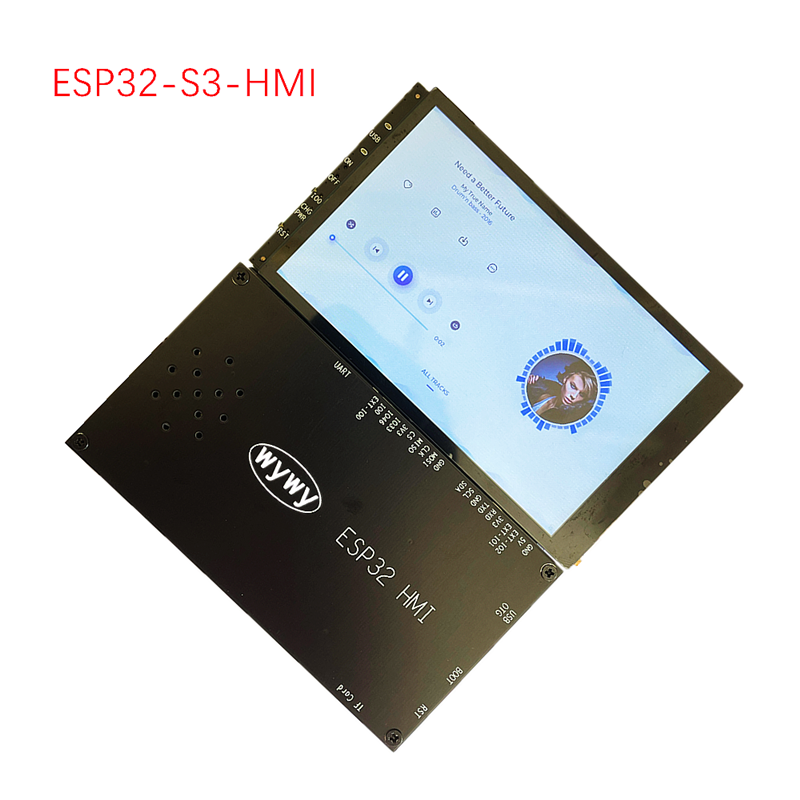
\includegraphics[width=0.3\textwidth]{Images/ESP32-S3-HMI-V3.png} 
  \caption{ESP32-S3-HMI-V3}
\end{figure}
\subsection{Cấu hình phần cứng của mô-đun ESP32-S3-HMI-V3} 
\tab Trung tâm xử lý của mô-đun là vi điều khiển ESP32-S3 do Espressif phát triển, sử dụng kiến trúc dual-core Xtensa LX7, hoạt động ở tần số lên đến 240MHz. Vi xử lý này được trang bị các tập lệnh SIMD và phần cứng tăng tốc AI giúp tăng cường khả năng xử lý tín hiệu số và các tác vụ học máy ngay tại thiết bị mà không cần gửi dữ liệu lên máy chủ.\\
\tab Mô-đun được tích hợp màn hình cảm ứng điện dung kích thước 2.8 inch (hoặc tùy chọn 4.3 inch tùy phiên bản), sử dụng tấm nền IPS với độ phân giải 320x240 (hoặc 800x480). Màn hình này được điều khiển bởi chip ST7789V hoặc ILI9488, kết nối qua giao tiếp SPI tốc độ cao, cho phép hiển thị giao diện người dùng sắc nét và mượt mà, đặc biệt phù hợp với các thư viện đồ họa như LVGL.\\
\tab Ngoài bộ nhớ trong 512KB SRAM và 384KB ROM tích hợp trên vi điều khiển ESP32-S3, mô-đun còn hỗ trợ mở rộng bộ nhớ ngoài với flash SPI 8MB và PSRAM 8MB. Đây là yếu tố quan trọng cho các ứng dụng đồ họa hoặc xử lý AI, giúp lưu trữ hình ảnh, giao diện và dữ liệu tạm thời với tốc độ truy cập nhanh.\\
\tab Mô-đun còn có sẵn khe cắm thẻ TF (microSD), giao tiếp USB Type-C hỗ trợ USB-OTG và debug UART, cùng các chân mở rộng GPIO qua header 2.54mm, hỗ trợ kết nối với cảm biến, thiết bị đầu cuối hoặc các mô-đun mở rộng khác. Ngoài ra, hệ thống còn tích hợp mạch sạc pin Li-ion/Li-Po và bảo vệ nguồn, thích hợp cho các ứng dụng di động hoặc thiết bị không dây dùng pin.
\begin{figure}[H]
  \centering
  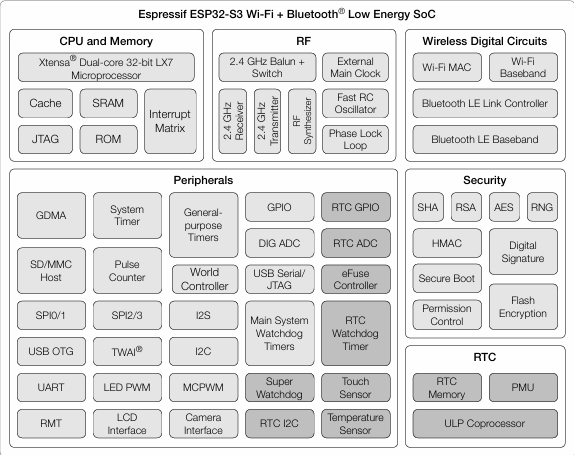
\includegraphics[width=0.6\textwidth]{Images/ESP32-S3-Funtion-diagram.png} 
  \caption{ESP32-S3 Functional Block Diagram}
\end{figure}
\subsection{Khả năng kết nối và truyền thông} 
\tab ESP32-S3-HMI-V3 hỗ trợ đầy đủ các chuẩn kết nối không dây hiện đại thông qua Wi-Fi 802.11 b/g/n và Bluetooth 5.0 LE. Điều này cho phép mô-đun dễ dàng tích hợp vào hệ thống mạng nội bộ hoặc điều khiển từ xa qua internet, phù hợp với các ứng dụng như điều khiển nhà thông minh, cập nhật firmware OTA hoặc đồng bộ dữ liệu thời gian thực với server.\\
\tab Mô-đun cũng hỗ trợ các giao thức truyền thông phổ biến như UART, SPI, I2C và RS485 (qua chip mở rộng), giúp giao tiếp dễ dàng với cảm biến, thiết bị ngoại vi và hệ thống SCADA công nghiệp. Giao tiếp RS485 đặc biệt quan trọng trong môi trường công nghiệp, nơi tín hiệu cần truyền đi xa và chống nhiễu tốt.
\subsection{Hỗ trợ phần mềm và phát triển ứng dụng} 
\tab ESP32-S3-HMI-V3 được hỗ trợ chính thức bởi ESP-IDF, bộ SDK mạnh mẽ của Espressif, tích hợp FreeRTOS, các thư viện giao tiếp mạng, AI và hỗ trợ thư viện đồ họa như LVGL để xây dựng giao diện người dùng hiện đại. Việc sử dụng LVGL giúp phát triển nhanh chóng các màn hình cảm ứng với button, menu, slider, biểu đồ v.v. mà không cần tự vẽ từng pixel.\\
\tab Đối với người dùng Arduino, mô-đun này cũng tương thích với Arduino IDE thông qua bộ lõi ESP32-S3, cho phép viết code nhanh chóng bằng ngôn ngữ Arduino, sử dụng các thư viện như TFT\_eSPI hoặc LovyanGFX để điều khiển màn hình.\\

\tab Mô-đun còn hỗ trợ lập trình bằng MicroPython – một lựa chọn tuyệt vời cho những ứng dụng nhẹ, dạy học, hoặc triển khai nhanh mẫu thử (prototype). Ngoài ra, mô-đun tương thích với các công cụ debug nâng cao như JTAG, OpenOCD thông qua USB hoặc header mở rộng.
\subsection{Ứng dụng thực tế} 
\tab Nhờ tích hợp màn hình cảm ứng, khả năng kết nối đa dạng, hiệu năng xử lý mạnh và hỗ trợ AI, mô-đun ESP32-S3-HMI-V3 được sử dụng rộng rãi trong các ứng dụng như:
\begin{itemize} 
\item Hệ thống điều khiển giám sát công nghiệp (HMI Panel) 
\item Màn hình cảm ứng cho thiết bị điện thông minh (bảng điều khiển đèn, máy lạnh, cửa cuốn) 
\item Giao diện cho thiết bị IoT trong nông nghiệp, y tế, logistics 
\item Thiết bị cầm tay với màn hình cảm ứng dùng pin 
\item Thiết bị nhận diện khuôn mặt, nhận diện âm thanh hoặc các hệ thống nhúng sử dụng AI 
\end{itemize}
\section{Cơ sở lý thuyết về module RS485}
\subsection{Giới thiệu chung về module RS485} 
\tab Module RS485 là một thiết bị trung gian giúp chuyển đổi tín hiệu UART (TTL) từ vi điều khiển sang chuẩn truyền thông RS485, cho phép giao tiếp trong các hệ thống truyền dữ liệu công nghiệp hoặc khoảng cách xa. Các module này thường được tích hợp sẵn mạch điện trở kéo, bảo vệ điện áp và mạch truyền nhận để đảm bảo tín hiệu ổn định và an toàn trong quá trình truyền thông.\\
\tab RS485 hỗ trợ giao tiếp đa điểm (multi-point), cho phép kết nối nhiều thiết bị với nhau trên cùng một đường truyền dữ liệu (bus), giúp đơn giản hóa hệ thống dây và giảm chi phí triển khai trong các ứng dụng như hệ thống giám sát, tự động hóa tòa nhà, mạng cảm biến môi trường, v.v.
\begin{figure}[H]
  \centering
  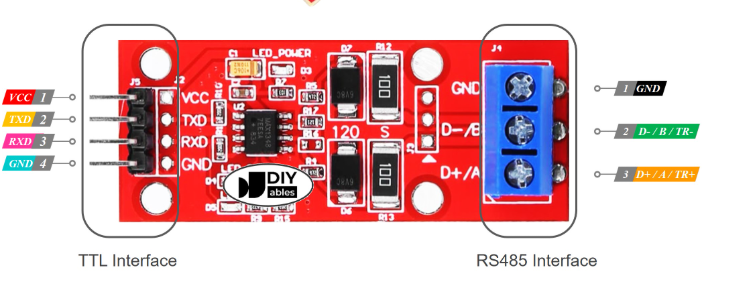
\includegraphics[width=0.6\textwidth]{Images/RS485.png}
  \caption{RS485 module}
\end{figure}
\subsection{Nguyên lý hoạt động của module RS485} 
\tab Module RS485 hoạt động dựa trên nguyên lý truyền vi sai (differential signaling), sử dụng hai dây tín hiệu chính là A và B. Tín hiệu được truyền dưới dạng chênh lệch điện áp giữa hai dây này thay vì so với mass như các chuẩn UART hay RS232 thông thường. Khi mức điện áp trên chân A cao hơn B (A > B), tín hiệu được xem là logic "1", ngược lại nếu A < B thì là logic "0". Điều này giúp loại bỏ nhiễu điện từ chung trên đường truyền và duy trì tính toàn vẹn dữ liệu.\\
\tab Các module RS485 phổ biến hiện nay sử dụng IC chuyển đổi như MAX485, SP485, hoặc SN75176 để thực hiện quá trình mã hóa và giải mã tín hiệu vi sai. Các IC này thường hỗ trợ cả chế độ truyền và nhận (half-duplex), và cần thêm một chân điều khiển (thường là DE/RE) để chuyển đổi giữa hai chế độ.

\subsection{Kết nối với vi điều khiển (ví dụ ESP32-S3)} 
\tab Việc kết nối module RS485 với vi điều khiển như ESP32-S3 thường thông qua giao tiếp UART. Các chân TX và RX của vi điều khiển được nối với module RS485 thông qua mạch chuyển đổi mức tín hiệu. Ngoài ra, chân DE (Driver Enable) và RE (Receiver Enable) thường được điều khiển bằng phần mềm để bật chế độ truyền hoặc nhận dữ liệu. Trong nhiều module, DE và RE được nối với nhau và điều khiển chung qua một chân GPIO của vi điều khiển để đơn giản hóa việc lập trình.\\
\tab Ví dụ, để gửi dữ liệu, chân DE/RE được đặt ở mức HIGH để bật chế độ truyền. Sau khi gửi xong, chân này sẽ được kéo xuống mức LOW để chuyển sang chế độ nhận. Thời điểm chuyển trạng thái cần được lập trình chính xác để tránh mất dữ liệu hoặc xung đột đường truyền.

\subsection{Ứng dụng thực tế} 
\tab Module RS485 được sử dụng rộng rãi trong nhiều ứng dụng yêu cầu truyền thông ổn định ở khoảng cách xa như: 
\begin{itemize} 
  \item Giao tiếp giữa các bộ điều khiển khả trình (PLC) và cảm biến/thiết bị chấp hành. 
  \item Mạng Modbus RTU trong hệ thống SCADA. 
  \item Mạng cảm biến trong nhà máy, nông nghiệp thông minh, hoặc giám sát năng lượng. 
  \item Hệ thống đo đạc từ xa như đồng hồ điện, nước, và hệ thống kiểm soát truy cập. 
\end{itemize} 
\tab Với khả năng chống nhiễu tốt, chi phí thấp và triển khai dễ dàng, module RS485 là lựa chọn lý tưởng cho các hệ thống truyền thông công nghiệp và IoT.

\section{MQTT trong IoT}

\subsection{Tổng quan về MQTT}

MQTT (Message Queuing Telemetry Transport) là một giao thức truyền thông nhẹ, được thiết kế tối ưu cho các ứng dụng có băng thông thấp, độ trễ cao hoặc yêu cầu tiêu thụ năng lượng thấp — đặc điểm điển hình trong các hệ thống Internet of Things (IoT). Giao thức này hoạt động theo mô hình \textbf{publish/subscribe} (xuất bản/đăng ký), cho phép các thiết bị trao đổi dữ liệu thông qua một máy chủ trung gian gọi là \textbf{broker}.

MQTT ban đầu được phát triển bởi IBM vào năm 1999 và hiện nay là một chuẩn mở, được quản lý bởi tổ chức OASIS (Organization for the Advancement of Structured Information Standards).
\begin{figure}[H]
  \centering
  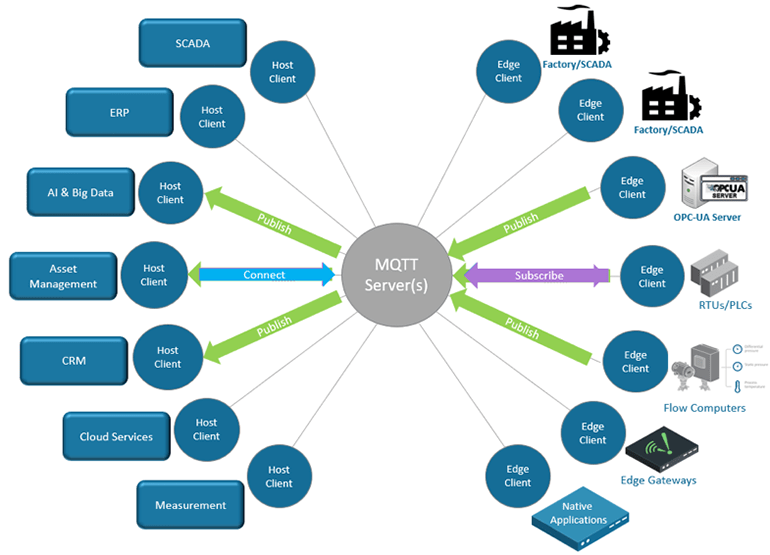
\includegraphics[width=0.6\textwidth]{Images/MQTT-trong-IoT.png}
  \caption{MQTT trong IoT}
\end{figure}
\subsection{Kiến trúc MQTT}

Kiến trúc MQTT bao gồm ba thành phần chính:

\begin{itemize}
    \item \textbf{Publisher (Thiết bị xuất bản):} Gửi thông điệp đến một chủ đề (topic) cụ thể.
    \item \textbf{Subscriber (Thiết bị đăng ký):} Nhận thông điệp bằng cách đăng ký các chủ đề quan tâm.
    \item \textbf{Broker (Máy chủ trung gian):} Tiếp nhận các thông điệp từ publisher và phân phối chúng đến các subscriber phù hợp. Ví dụ broker phổ biến: Mosquitto, HiveMQ, EMQX.
\end{itemize}
\begin{figure}[H]
  \centering
  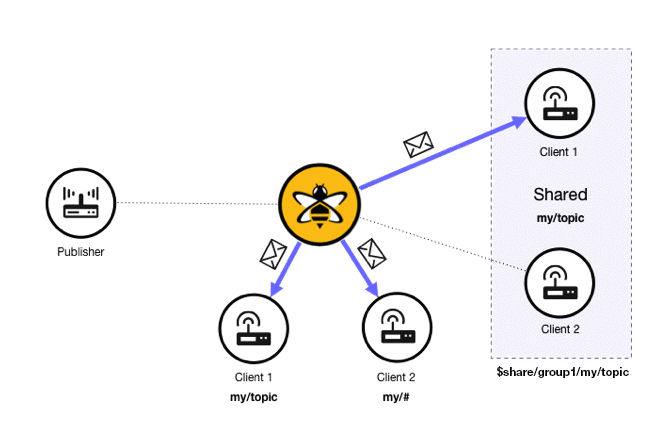
\includegraphics[width=0.6\textwidth]{Images/mo-hinh-mqtt.png}
  \caption{Mô hình Publish/Subscriber trong giao thức MQTT}
\end{figure}
\subsection{Nguyên lý hoạt động}

Khi một thiết bị \textbf{publisher} gửi một thông điệp (message) đến một \textbf{topic}, \textbf{broker} sẽ tiếp nhận thông điệp và phân phối nó đến tất cả các thiết bị \textbf{subscriber} đã đăng ký với topic đó. Giao thức MQTT cho phép hệ thống mở rộng dễ dàng và giảm đáng kể độ phụ thuộc giữa các thiết bị đầu cuối.

Ví dụ:
\begin{itemize}
    \item Publisher gửi dữ liệu cảm biến đến topic \texttt{``/home/temperature''}.
    \item Tất cả các subscriber quan tâm đến chủ đề này sẽ nhận được dữ liệu mà không cần biết thông tin về publisher.
\end{itemize}
\begin{figure}[H]
  \centering
  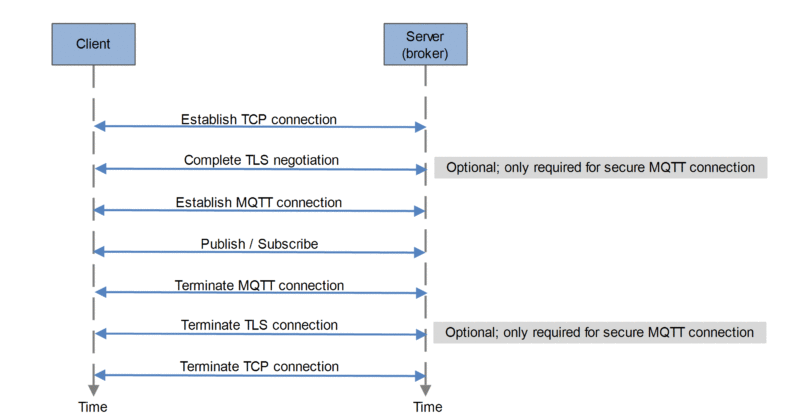
\includegraphics[width=0.8\textwidth]{Images/mqtt-data-1.png}
  \caption{Cơ chế hoạt động của giao thức MQTT}
\end{figure}
\subsection{Cấu trúc topic}

Topic trong MQTT được tổ chức theo dạng cây, sử dụng dấu gạch chéo \texttt{/} để phân tách các cấp.

Ví dụ:
\begin{itemize}
    \item \texttt{/home/livingroom/temperature}
    \item \texttt{/device/esp32/status}
\end{itemize}

MQTT hỗ trợ ký tự đại diện:
\begin{itemize}
    \item \texttt{+} đại diện cho một cấp (level).
    \item \texttt{\#} đại diện cho nhiều cấp (từ vị trí hiện tại trở đi).
\end{itemize}

\subsection{Chất lượng dịch vụ (QoS)}

MQTT hỗ trợ ba mức độ đảm bảo chất lượng dịch vụ (Quality of Service - QoS):

\begin{itemize}
    \item \textbf{QoS 0 - At most once:} Gửi một lần và không đảm bảo nhận được.
    \item \textbf{QoS 1 - At least once:} Gửi ít nhất một lần, có thể trùng lặp.
    \item \textbf{QoS 2 - Exactly once:} Gửi đúng một lần (đảm bảo không trùng và không mất).
\end{itemize}

\subsection{Ứng dụng của MQTT trong IoT}

MQTT được sử dụng rộng rãi trong nhiều hệ thống IoT nhờ vào tính nhẹ, đơn giản và hiệu quả:

\begin{itemize}
    \item \textbf{Nhà thông minh (Smart home):} Kết nối thiết bị đèn, cảm biến, điều hòa.
    \item \textbf{Nông nghiệp thông minh:} Gửi dữ liệu độ ẩm, nhiệt độ, mực nước về máy chủ.
    \item \textbf{Giám sát công nghiệp:} Truyền dữ liệu cảm biến từ xa về trung tâm điều khiển.
    \item \textbf{Thiết bị đeo và sức khỏe:} Đồng bộ hóa dữ liệu sức khỏe với cloud server.
\end{itemize}
\begin{figure}[H]
  \centering
  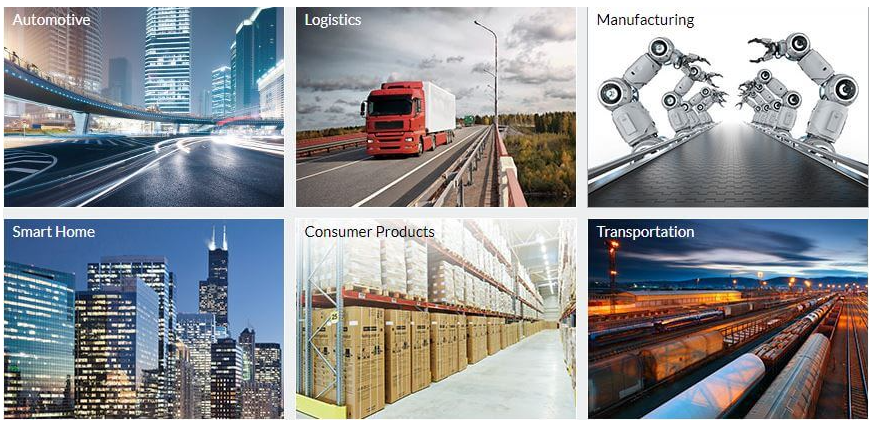
\includegraphics[width=0.6\textwidth]{Images/ung-dung-mqtt.png}
  \caption{Ứng dụng của MQTT trong IoT}
\end{figure}
\subsection{Ưu và nhược điểm của MQTT}

\textbf{Ưu điểm:}
\begin{itemize}
    \item Giao thức nhẹ, phù hợp với thiết bị tài nguyên hạn chế.
    \item Giao tiếp không đồng bộ và tách biệt giữa publisher và subscriber.
    \item Hỗ trợ nhiều mức QoS và cơ chế giữ kết nối (keep-alive).
\end{itemize}

\textbf{Nhược điểm:}
\begin{itemize}
    \item Phụ thuộc vào broker trung gian.
    \item Không mã hóa mặc định, cần kết hợp với SSL/TLS để đảm bảo an toàn.
    \item Không phù hợp với các ứng dụng yêu cầu thời gian thực chính xác tuyệt đối.
\end{itemize}

\section{Thư viện đồ họa LVGL}
\tab LVGL (Light and Versatile Graphics Library) là một thư viện đồ họa mã nguồn mở, nhẹ nhàng và linh hoạt, được thiết kế đặc biệt cho các hệ thống nhúng với tài nguyên hạn chế. Thư viện này cung cấp tất cả các công cụ cần thiết để tạo ra giao diện người dùng đồ họa (GUI) hấp dẫn và chuyên nghiệp trên các vi điều khiển như ESP32, với hiệu suất tối ưu và yêu cầu bộ nhớ thấp.
\subsection{Tổng quan về LVGL}
\tab LVGL được phát triển từ năm 2016 bởi Gábor Kiss-Vámosi, ban đầu với tên gọi LittlevGL. Qua nhiều năm phát triển, LVGL đã trở thành một trong những thư viện GUI phổ biến nhất cho các hệ thống nhúng, với các phiên bản chính từ v5 đến v9 hiện nay. Mỗi phiên bản đều mang đến những cải tiến đáng kể về hiệu suất, tính năng và khả năng tương thích.\\
\tab LVGL có nhiều đặc điểm và ưu điểm nổi bật so với các thư viện đồ họa khác cho hệ thống nhúng. Thư viện này được thiết kế với kiến trúc module hóa, cho phép chỉ biên dịch các thành phần cần thiết, giảm thiểu kích thước mã nguồn. LVGL hỗ trợ đa nền tảng, có thể chạy trên hầu hết các vi điều khiển 16, 32 hoặc 64 bit, từ các chip đơn giản như STM32 đến các nền tảng mạnh mẽ hơn như ESP32 hoặc Raspberry Pi.\\
\tab Một trong những ưu điểm lớn nhất của LVGL là khả năng tạo ra giao diện người dùng hiện đại và hấp dẫn với yêu cầu tài nguyên tối thiểu. Thư viện có thể hoạt động với chỉ 64 KB flash và 16 KB RAM, mặc dù cấu hình được khuyến nghị là khoảng 180 KB flash và 48 KB RAM để sử dụng đầy đủ tính năng. LVGL cũng hỗ trợ hoạt động với chỉ một frame buffer, giảm thiểu yêu cầu bộ nhớ đồng thời vẫn duy trì hiệu ứng đồ họa mượt mà.\\
\tab Về yêu cầu hệ thống và tương thích, LVGL có thể hoạt động trên hầu hết các vi điều khiển với tốc độ xung nhịp từ 16 MHz trở lên, mặc dù khuyến nghị tối thiểu 32 MHz cho hiệu suất tốt. Thư viện hỗ trợ nhiều loại màn hình với độ sâu màu khác nhau, từ màn hình đơn sắc đến màn hình TFT màu 16 hoặc 24 bit. LVGL cũng tương thích với nhiều loại thiết bị đầu vào như màn hình cảm ứng, nút bấm, encoder, và bàn phím.
\subsection{Kiến trúc LVGL}
\tab LVGL được xây dựng với kiến trúc module hóa, bao gồm các thành phần cốt lõi và các module chức năng. Cấu trúc này cho phép tùy chỉnh và mở rộng linh hoạt, đồng thời duy trì hiệu suất tối ưu cho các hệ thống nhúng.\\
\tab Cấu trúc lõi của LVGL bao gồm các module cơ bản như hệ thống đối tượng, quản lý bộ nhớ, hệ thống sự kiện, và engine vẽ. Các module này tạo nền tảng cho toàn bộ thư viện và cung cấp các chức năng cơ bản như quản lý đối tượng, xử lý sự kiện, và render đồ họa. LVGL sử dụng kiến trúc hướng đối tượng mặc dù được viết bằng C, với các cấu trúc dữ liệu và hàm được tổ chức theo cách mô phỏng lập trình hướng đối tượng.\\
\tab Hệ thống đối tượng và thừa kế trong LVGL cho phép tạo ra các widget phức tạp từ các thành phần cơ bản. Mỗi đối tượng trong LVGL đều kế thừa từ lớp cơ sở \texttt{lv\_obj}, thừa hưởng các thuộc tính và phương thức của lớp cha, đồng thời có thể mở rộng với các chức năng riêng. Cơ chế thừa kế này giúp giảm thiểu mã lặp lại và tạo ra hệ thống widget nhất quán và dễ mở rộng.\\
\tab Cơ chế quản lý bộ nhớ trong LVGL được thiết kế đặc biệt cho các hệ thống nhúng với bộ nhớ hạn chế. LVGL sử dụng bộ cấp phát bộ nhớ động riêng, cho phép kiểm soát chặt chẽ việc sử dụng bộ nhớ và tránh phân mảnh. Thư viện cũng hỗ trợ các cơ chế tái sử dụng bộ nhớ và giải phóng tự động, giảm thiểu rò rỉ bộ nhớ và tối ưu hóa hiệu suất.\\
\tab Hệ thống sự kiện và callback trong LVGL cho phép xử lý tương tác người dùng một cách linh hoạt và hiệu quả. Mỗi đối tượng có thể đăng ký các hàm callback để phản hồi với các sự kiện như nhấn, kéo, hoặc thay đổi giá trị. Hệ thống sự kiện hỗ trợ lan truyền sự kiện qua cây đối tượng, cho phép xử lý sự kiện ở nhiều cấp độ khác nhau.
\begin{figure}[H]
  \centering
  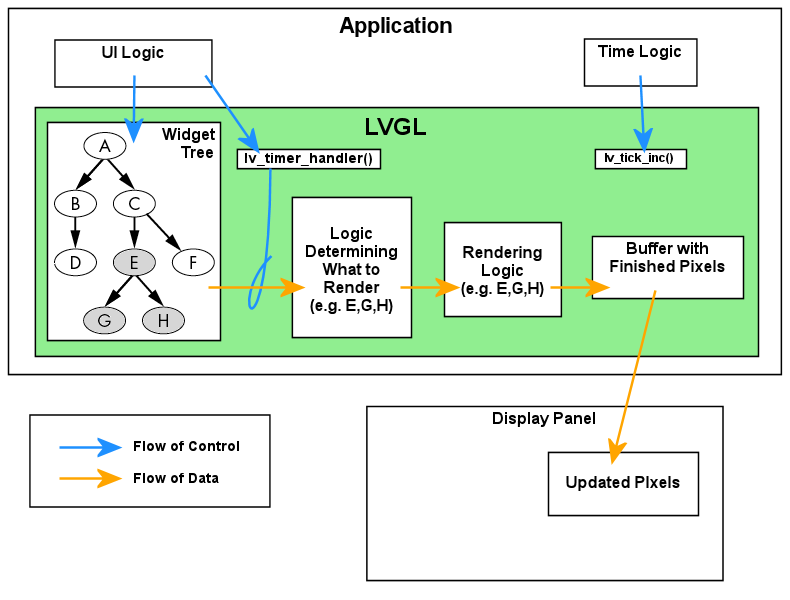
\includegraphics[width=0.6\textwidth]{Images/LGVL_intro_data_flow.png}
  \caption{Tổng quan về luồng dữ liệu của LVGL}
\end{figure}
\subsection{Các thành phần chính giao diện}
\tab LVGL cung cấp một bộ widget phong phú để xây dựng giao diện người dùng, từ các thành phần cơ bản đến các container phức tạp và hệ thống bố cục linh hoạt.\\
Hệ thống widget cơ bản của LVGL bao gồm các thành phần như Button (nút bấm), Label (nhãn), và Image (hình ảnh). Button cung cấp chức năng tương tác cơ bản, với hỗ trợ cho các trạng thái khác nhau như nhấn, thả, và vô hiệu hóa. Label cho phép hiển thị văn bản với nhiều tùy chọn về font, căn chỉnh, và cuộn. Image hỗ trợ nhiều định dạng hình ảnh, bao gồm cả hình ảnh nén và hình ảnh với kênh alpha.\\
\tab Ngoài các widget cơ bản, LVGL còn cung cấp các thành phần phức tạp hơn như Chart (biểu đồ), Table (bảng), Dropdown (danh sách thả xuống), và Keyboard (bàn phím ảo). Các widget này cho phép xây dựng giao diện người dùng phức tạp với ít mã nguồn hơn, đồng thời duy trì hiệu suất tốt trên các hệ thống nhúng.\\
\tab Hệ thống styles và themes trong LVGL cho phép tùy chỉnh giao diện một cách linh hoạt và nhất quán. Styles định nghĩa các thuộc tính như màu sắc, font, padding, và border cho các widget. LVGL sử dụng cơ chế CSS-like để áp dụng styles, cho phép kế thừa và ghi đè các thuộc tính. Themes là tập hợp các styles được định nghĩa sẵn, cung cấp giao diện nhất quán cho toàn bộ ứng dụng.\\
\tab Bố cục và container trong LVGL giúp tổ chức các widget một cách linh hoạt và phản ứng. LVGL hỗ trợ các hệ thống bố cục hiện đại như Flex (dựa trên CSS Flexbox) và Grid (dựa trên CSS Grid), cho phép tạo ra giao diện phản ứng tự động điều chỉnh theo kích thước màn hình. Các container như Panel, Tabview, và Window giúp tổ chức nội dung thành các phần logic và cung cấp các chức năng như cuộn và chuyển tab.\\
\tab Hiệu ứng đồ họa và animation trong LVGL mang lại trải nghiệm người dùng động và hấp dẫn. Thư viện hỗ trợ các hiệu ứng như fade, move, và scale, với khả năng tùy chỉnh thời gian, đường cong chuyển động, và callback. Animations có thể được áp dụng cho hầu hết các thuộc tính của widget, từ vị trí và kích thước đến màu sắc và độ trong suốt.
\section{Công nghệ hiển thị cho hệ thống nhúng}
\tab Công nghệ hiển thị đóng vai trò quan trọng trong việc phát triển giao diện người dùng cho các hệ thống nhúng như ESP32. Các loại màn hình khác nhau cung cấp nhiều tùy chọn về kích thước, độ phân giải, chất lượng hiển thị và phương thức giao tiếp, cho phép nhà phát triển lựa chọn giải pháp phù hợp nhất với yêu cầu của dự án.
\subsection{Màn hình LCD và TFT}
\tab Màn hình LCD (Liquid Crystal Display) và đặc biệt là công nghệ TFT (Thin Film Transistor) LCD đã trở thành lựa chọn phổ biến cho các ứng dụng nhúng nhờ khả năng hiển thị màu sắc sống động, độ phân giải cao và giá thành hợp lý.\\
\tab Nguyên lý hoạt động của màn hình LCD dựa trên việc điều khiển các tinh thể lỏng để thay đổi cách ánh sáng đi qua chúng. Mỗi điểm ảnh (pixel) trên màn hình LCD bao gồm các tinh thể lỏng được đặt giữa hai tấm phân cực. Khi áp dụng điện áp, các tinh thể lỏng xoay và thay đổi cách ánh sáng đi qua, tạo ra các mức độ sáng tối khác nhau. Trong màn hình TFT LCD, mỗi pixel được điều khiển bởi một hoặc nhiều transistor màng mỏng, cho phép điều khiển độc lập và cải thiện đáng kể chất lượng hiển thị so với LCD thông thường.\\
\tab Các loại màn hình phổ biến cho ESP32 bao gồm ILI9341 và ST7789. Màn hình ILI9341 thường có kích thước 2.8 inch với độ phân giải 240x320 pixel, trong khi ST7789 thường được sử dụng trong các màn hình có kích thước từ 1.3 đến 2.0 inch với độ phân giải tương tự. Cả hai loại controller này đều hỗ trợ giao tiếp SPI, cho phép kết nối dễ dàng với ESP32 và tiêu thụ ít chân GPIO.\\
\tab Các đặc tính kỹ thuật quan trọng của màn hình TFT LCD bao gồm độ phân giải, độ sâu màu, góc nhìn và tốc độ làm mới. Độ phân giải thông thường cho các màn hình nhỏ dao động từ 240x240 đến 480x320 pixel. Độ sâu màu thường là 16-bit (65,536 màu) hoặc 18-bit (262,144 màu). Các yếu tố như góc nhìn và độ sáng cũng đóng vai trò quan trọng đối với trải nghiệm người dùng.

\subsection{Màn hình OLED}
\tab Màn hình OLED (Organic Light Emitting Diode) là công nghệ hiển thị tiên tiến với nhiều ưu điểm so với LCD, đặc biệt phù hợp cho các ứng dụng nhúng yêu cầu tiết kiệm năng lượng và chất lượng hiển thị cao.\\
\tab Nguyên lý hoạt động của màn hình OLED dựa trên các diode phát quang hữu cơ có khả năng tự phát sáng khi có dòng điện đi qua. Mỗi pixel là một diode phát quang độc lập, không cần đèn nền. Điều này cho phép tỷ lệ tương phản cao, thời gian đáp ứng nhanh, góc nhìn rộng và tiêu thụ năng lượng thấp khi hiển thị nội dung tối.\\
\tab So với LCD/TFT, OLED có tỷ lệ tương phản và độ sống động màu sắc cao hơn, thời gian đáp ứng nhanh hơn (dưới 1ms), và tiêu thụ năng lượng thấp hơn. Tuy nhiên, OLED có tuổi thọ ngắn hơn, dễ bị hiện tượng burn-in và chi phí cao hơn.\\
\tab Trong hệ thống nhúng, OLED phù hợp cho thiết bị đeo, thiết bị y tế cầm tay và các thiết bị IoT chạy pin. Nó cũng là lựa chọn lý tưởng trong môi trường ánh sáng yếu.
\subsection{Giao tiếp với màn hình}
Giao tiếp giữa ESP32 và màn hình là yếu tố ảnh hưởng đến hiệu suất và độ phức tạp của hệ thống. Các giao thức phổ biến gồm SPI, I2C và giao tiếp song song.

\begin{itemize}
  \item \textbf{SPI (Serial Peripheral Interface):} phổ biến cho màn hình TFT và OLED. Giao thức này sử dụng các đường MOSI, MISO, SCK và CS, có tốc độ cao (lên đến 80MHz). ESP32 có thể dùng DMA để cải thiện hiệu suất truyền dữ liệu.
  
  \item \textbf{I2C (Inter-Integrated Circuit):} phù hợp với màn hình OLED nhỏ và controller cảm ứng. Chỉ sử dụng hai dây SDA và SCL, giúp tiết kiệm GPIO. Nhược điểm là tốc độ thấp hơn (100kHz đến 1MHz).
  
  \item \textbf{Giao tiếp song song (Parallel):} cung cấp băng thông cao nhất nhưng cần nhiều GPIO. Giao tiếp 8-bit hoặc 16-bit được hỗ trợ qua giao diện I8080/6800.
\end{itemize}

Về điều khiển cảm ứng, các controller như XPT2046 (cảm ứng điện trở) và FT6X36 (cảm ứng điện dung) sử dụng SPI hoặc I2C. Cảm ứng điện dung hỗ trợ multi-touch và có trải nghiệm tốt hơn, nhưng phức tạp và đắt hơn cảm ứng điện trở.

Việc lựa chọn công nghệ hiển thị và phương thức giao tiếp phù hợp là yếu tố then chốt để tạo ra giao diện người dùng hiệu quả trên nền tảng ESP32. Kết hợp với thư viện như LVGL sẽ nâng cao trải nghiệm người dùng.

\section{Phân tích các giải pháp GUI cho ESP32}
\tab Khi phát triển ứng dụng với giao diện đồ họa người dùng (GUI) cho ESP32, nhà phát triển có nhiều lựa chọn về thư viện đồ họa. Mỗi thư viện có những ưu điểm, nhược điểm và trường hợp sử dụng riêng. Việc phân tích và so sánh các giải pháp này giúp lựa chọn công cụ phù hợp nhất cho dự án cụ thể.
\subsection{Các thư viện đồ họa hiện có}
\tab Thị trường thư viện đồ họa cho ESP32 khá đa dạng, với nhiều lựa chọn từ các thư viện đơn giản, nhẹ nhàng đến các framework GUI toàn diện. Dưới đây là phân tích chi tiết về các thư viện phổ biến nhất.
\subsubsection{TFT\_eSPI (Bodmer)}
\tab TFT\_eSPI là một thư viện đồ họa mạnh mẽ và được tối ưu hóa cao cho ESP32 và các vi điều khiển khác, được phát triển bởi Bodmer. Thư viện này được thiết kế đặc biệt cho màn hình TFT sử dụng giao tiếp SPI.\\
\tab Ưu điểm chính của TFT\_eSPI bao gồm hiệu suất cao nhờ tối ưu hóa mã assembly và sử dụng DMA, hỗ trợ nhiều loại controller màn hình (ILI9341, ST7789, ILI9488, \ldots), và tích hợp tốt với hệ sinh thái Arduino. Thư viện cung cấp các hàm vẽ cơ bản như điểm, đường, hình chữ nhật, hình tròn, và văn bản, cùng với hỗ trợ hiển thị hình ảnh và sprite (đối tượng đồ họa có thể di chuyển).\\
\tab Tuy nhiên, TFT\_eSPI có một số hạn chế. Thư viện không cung cấp các widget GUI cao cấp như nút bấm, thanh trượt, hoặc menu, khiến việc xây dựng giao diện người dùng phức tạp trở nên khó khăn hơn. Cấu hình thư viện cũng khá phức tạp, đòi hỏi chỉnh sửa file \texttt{User\_Setup.h} để phù hợp với phần cứng cụ thể.\\
\tab TFT\_eSPI phù hợp nhất cho các ứng dụng yêu cầu hiệu suất cao, hiển thị đồ họa cơ bản, hoặc khi nhà phát triển muốn xây dựng GUI tùy chỉnh từ đầu.
\subsubsection{Adafruit GFX}
\tab Adafruit GFX là một thư viện đồ họa phổ biến và dễ sử dụng, được phát triển bởi Adafruit Industries. Thư viện này cung cấp một API nhất quán cho nhiều loại màn hình khác nhau, từ OLED đơn sắc đến TFT màu.\\
\tab Ưu điểm của Adafruit GFX bao gồm tính đơn giản và dễ học, hỗ trợ rộng rãi từ cộng đồng, và tương thích với nhiều loại màn hình thông qua các thư viện driver riêng (như \texttt{Adafruit\_ILI9341}, \texttt{Adafruit\_SSD1306}). Thư viện cung cấp các hàm vẽ cơ bản tương tự như TFT\_eSPI, cùng với hỗ trợ font và hiển thị bitmap.\\
\tab Tuy nhiên, Adafruit GFX không được tối ưu hóa cho hiệu suất cao như TFT\_eSPI, đặc biệt trên ESP32. Thư viện cũng thiếu các widget GUI và hệ thống quản lý sự kiện, đòi hỏi nhà phát triển phải xây dựng các thành phần này từ đầu.\\
\tab Adafruit GFX là lựa chọn tốt cho người mới bắt đầu, các dự án đơn giản, hoặc khi cần tương thích với nhiều loại màn hình khác nhau trong cùng một codebase.
\subsubsection{U8g2}
\tab U8g2 là một thư viện đồ họa monochrome (đơn sắc) được tối ưu hóa cho các màn hình OLED và LCD đơn sắc. Mặc dù chủ yếu tập trung vào hiển thị đơn sắc, U8g2 vẫn là một lựa chọn quan trọng trong hệ sinh thái ESP32.\\
\tab Ưu điểm của U8g2 bao gồm kích thước nhỏ gọn, tiêu thụ bộ nhớ thấp, và hỗ trợ rộng rãi cho các controller màn hình đơn sắc (SSD1306, SH1106, \ldots). Thư viện cung cấp nhiều font với kích thước khác nhau, hỗ trợ nhiều ngôn ngữ, và có cơ chế buffer kép để tránh hiện tượng nhấp nháy khi cập nhật màn hình.\\
\tab Hạn chế chính của U8g2 là chỉ hỗ trợ màn hình đơn sắc, không phù hợp cho các ứng dụng yêu cầu hiển thị màu. Thư viện cũng thiếu các widget GUI và hệ thống quản lý sự kiện như các thư viện khác.\\
\tab U8g2 là lựa chọn tuyệt vời cho các ứng dụng sử dụng màn hình OLED đơn sắc, đặc biệt khi tài nguyên hệ thống hạn chế hoặc khi tiêu thụ năng lượng là ưu tiên hàng đầu.
\subsubsection{LVGL}

LVGL (Light and Versatile Graphics Library) là một thư viện GUI toàn diện, cung cấp không chỉ các hàm vẽ cơ bản mà còn bao gồm hệ thống widget phong phú, quản lý sự kiện, và nhiều tính năng cao cấp khác.

Như đã phân tích chi tiết trong phần trước, LVGL có nhiều ưu điểm nổi bật so với các thư viện khác. Thư viện cung cấp bộ widget phong phú (nút bấm, thanh trượt, bảng, biểu đồ, \ldots), hệ thống styles và themes linh hoạt, và hỗ trợ animation. LVGL được thiết kế để hoạt động hiệu quả trên các hệ thống nhúng với tài nguyên hạn chế, yêu cầu chỉ 64\,KB flash và 16\,KB RAM cho các tính năng cơ bản.

LVGL cũng có khả năng mở rộng cao, cho phép nhà phát triển tạo ra các widget tùy chỉnh hoặc mở rộng các widget có sẵn. Thư viện hỗ trợ nhiều loại thiết bị đầu vào (cảm ứng, nút bấm, encoder) và có thể hoạt động với nhiều loại màn hình khác nhau thông qua hệ thống driver linh hoạt.

Tuy nhiên, LVGL có đường cong học tập dốc hơn so với các thư viện đơn giản như Adafruit GFX, và cấu hình ban đầu có thể phức tạp. Thư viện cũng yêu cầu nhiều tài nguyên hơn so với các giải pháp đơn giản hơn, mặc dù vẫn được tối ưu hóa cho hệ thống nhúng.

LVGL là lựa chọn lý tưởng cho các ứng dụng yêu cầu GUI phức tạp, chuyên nghiệp, với nhiều widget tương tác và hiệu ứng đồ họa.

\subsection{So sánh và lựa chọn thư viện phù hợp}

Khi lựa chọn thư viện đồ họa cho dự án ESP32, cần cân nhắc nhiều yếu tố khác nhau để đưa ra quyết định phù hợp nhất.

\subsubsection{Hiệu suất và tài nguyên}

Về hiệu suất render, TFT\_eSPI thường dẫn đầu nhờ tối ưu hóa assembly và sử dụng DMA, tiếp theo là LVGL với engine render được tối ưu hóa. Adafruit GFX và U8g2 có hiệu suất thấp hơn nhưng vẫn đủ cho nhiều ứng dụng.

Về tiêu thụ bộ nhớ, U8g2 là nhẹ nhất, tiếp theo là TFT\_eSPI và Adafruit GFX. LVGL yêu cầu nhiều bộ nhớ nhất, đặc biệt khi sử dụng nhiều widget và animation, nhưng vẫn được tối ưu hóa cho hệ thống nhúng.

\subsubsection{Tính năng và khả năng mở rộng}

LVGL dẫn đầu về tính năng với bộ widget phong phú, hệ thống styles, và animation. TFT\_eSPI cung cấp các tính năng đồ họa cơ bản mạnh mẽ nhưng thiếu widgets. Adafruit GFX và U8g2 tập trung vào các chức năng vẽ cơ bản.

Về khả năng mở rộng, LVGL có kiến trúc module hóa cho phép mở rộng dễ dàng. TFT\_eSPI cũng khá linh hoạt nhưng đòi hỏi nhiều công sức hơn để mở rộng. Adafruit GFX và U8g2 có khả năng mở rộng hạn chế hơn.

\subsubsection{Độ phức tạp và đường cong học tập}

Adafruit GFX có đường cong học tập thoải nhất, phù hợp cho người mới bắt đầu. U8g2 và TFT\_eSPI có độ phức tạp trung bình, trong khi LVGL có đường cong học tập dốc nhất do cung cấp nhiều tính năng và khái niệm phức tạp hơn.

\subsubsection{Hỗ trợ cộng đồng và tài liệu}

Tất cả bốn thư viện đều có cộng đồng người dùng lớn và tài liệu tốt. Adafruit GFX có lợi thế về hướng dẫn và ví dụ từ Adafruit. LVGL có tài liệu toàn diện nhất với hướng dẫn, ví dụ, và tài liệu tham khảo API đầy đủ. TFT\_eSPI và U8g2 cũng có tài liệu tốt và cộng đồng hỗ trợ tích cực.

\subsubsection{Trường hợp sử dụng phù hợp}
\begin{itemize}
    \item \textbf{TFT\_eSPI}: Phù hợp nhất cho các ứng dụng yêu cầu hiệu suất cao, hiển thị đồ họa cơ bản, hoặc khi tài nguyên hệ thống hạn chế nhưng vẫn cần hiển thị màu.
    \item \textbf{Adafruit GFX}: Lý tưởng cho người mới bắt đầu, các dự án đơn giản, hoặc khi cần tương thích với nhiều loại màn hình khác nhau.
    \item \textbf{U8g2}: Tốt nhất cho các ứng dụng sử dụng màn hình OLED đơn sắc, đặc biệt khi tiêu thụ năng lượng và bộ nhớ là ưu tiên.
    \item \textbf{LVGL}: Phù hợp nhất cho các ứng dụng yêu cầu GUI phức tạp, chuyên nghiệp, với nhiều widget tương tác và hiệu ứng đồ họa.
\end{itemize}
\subsection{Tại sao chọn LVGL cho dự án phát triển thư viện giao diện}
Sau khi phân tích các giải pháp GUI hiện có, LVGL nổi bật như một lựa chọn tối ưu cho việc phát triển thư viện giao diện cho ESP32 vì nhiều lý do.
\begin{itemize}
    \item \textbf{Tính năng phong phú}: LVGL cung cấp một bộ widget phong phú và hệ thống styles linh hoạt, cho phép tạo ra giao diện người dùng hấp dẫn và chuyên nghiệp mà không cần phát triển từ đầu. Điều này giúp tiết kiệm thời gian phát triển đáng kể và mang lại kết quả chất lượng cao hơn.
    \item \textbf{Hiệu suất tối ưu}: LVGL được tối ưu hóa cho các hệ thống nhúng như ESP32, cân bằng giữa tính năng phong phú và hiệu suất. Thư viện có thể hoạt động hiệu quả với tài nguyên hạn chế của ESP32, đồng thời vẫn cung cấp trải nghiệm người dùng mượt mà.
    \item \textbf{Khả năng mở rộng}: Kiến trúc module hóa của LVGL cho phép mở rộng và tùy chỉnh dễ dàng, lý tưởng cho việc phát triển thư viện giao diện tùy chỉnh. Nhà phát triển có thể xây dựng các widget mới hoặc mở rộng các widget có sẵn để đáp ứng nhu cầu cụ thể của dự án.
    \item \textbf{Hỗ trợ cộng đồng và tài liệu}: LVGL có cộng đồng người dùng lớn, tài liệu toàn diện, và được cập nhật thường xuyên. Điều này đảm bảo rằng thư viện giao diện được phát triển sẽ có nền tảng vững chắc và hỗ trợ lâu dài.
\end{itemize}
\tab Với những ưu điểm trên, LVGL là nền tảng lý tưởng để phát triển thư viện giao diện cho ESP32, cung cấp sự cân bằng tối ưu giữa tính năng, hiệu suất, và khả năng mở rộng.
\newpage



\nocite{*}
% \begin{center}
\setlength{\Urlmuskip}{0mu plus 1mu} % Ngắt dòng URL linh hoạt
\begin{thebibliography}{99}

% BOOK
\bibitem{feedback_system} Karl Johan Astrom, Richard M. Murray, \emph{Feedback Systems: An Introduction for Scientists and Engineers}, Princeton University Press, 2012.

\bibitem{intergral_lqr} A Joukhadar, I Hasan, A Alsabbagh, M Alkouzbary, \emph{Integral Lqr-Based 6dof Autonomous Quadrocopter Balancing System Control}, International Journal of Advanced Research in Artificial Intelligence, Vol. 4, No.5, 2015.

\bibitem{manual_tunning} Nur Hayati Sahrir, Mohd Ariffanan Mohd Basri, \emph{Modelling and Manual Tuning PID Controlof Quadcopter}, Control, Instrumentation and Mechatronics: Theory and Practice (pp.346-357).

\bibitem{calculus} Nguyễn Đình Huy, \emph{Giáo trình giải tích 1}, Đại học Quốc gia TP. Hồ Chí Minh, 2020.

\bibitem{MultiGyro} Faisal Iqbal, Hussamud Din, Byeungleul Lee, \emph{Single Drive Multi-Axis Gyroscope with High Dynamic Range, High Linearity and Wide Bandwidth}, Micromachines 2019, 10(6), 410.

\bibitem{LQR} Heja Cengiz, \emph{Quadcopter Modeling and Linear Quadratic Regulator Design Using Simulink}, Uppsala Universitet, 2024.

% ARTICLE
\bibitem{IAEME} Ha Quang Thinh Ngo, Thanh Phuong Nguyen, Hung Nguyen, "A COMPLETE COMPARISON TO DESIGN COMPLEMENTARY FILTER AND KALMAN FILTER FOR AERIAL VEHICLE", \emph{International Journal of Mechanical Engineering and Technology}, 2018.

\bibitem{robotics_contrl} Rio Ikhsan Alfian, Alfian Ma'arif, Sunardi Sunardi, "Noise Reduction in the Accelerometer and Gyroscope Sensor with the Kalman Filter Algorithm", \emph{Journal of Robotics and Control (JRC)}, 2021.

\bibitem{discretePID} Luis E. Romero, David F. Pozo, Jorge A. Rosales, "Quadcopter Stabilization by Using PID Controllers", \emph{ACADEMIA}, 2014.

\bibitem{gyrophone} Yan Michalevsky, Dan Boneh, "Gyrophone: Recognizing Speech from Gyroscope Signals", \emph{Proceedings of the 23rd USENIX Security Symposium}, 2014.
\bibitem{lqr_handout} Dennis Freeman, Kevin Chen "Linear quadratic regulator (LQR) control" Source: https://introcontrol.mit.edu/\_static/spring23/lectures/lec08a-handout.pdf.
% MISC
\bibitem{mpudatasheet} "MPU-6000 and MPU-6050 Product Specification Revision 3.4", 2013. Source: www.invensense.com.

\bibitem{Mpu_guide_code} "Hướng dẫn sử dụng cảm biến gia tốc MPU6050 với Arduino", 2023. Source: https://arduinokit.vn/huong-dan-su-dung-cam-bien-gia-toc-mpu6050-voi-arduino/.

\bibitem{tkinter} "tkinter — Python interface to Tcl/Tk". Source: https://docs.python.org /3/library/tkinter.html.

\bibitem{socket} "socket — Low-level networking interface". Source: https://docs.python.org /3/library/socket.html.

\bibitem{arduino} "Arduino Documentation". Source: https://docs.arduino.cc/.

\bibitem{ultraSonic} "Distance Measurement with an Ultrasonic Sensor HY-SRF05", 2017. Source: https://projecthub.arduino.cc/Nicholas\_N/distance-measurement-with-an-ultrasonic-sensor-hy-srf05-bf2923.

\bibitem{escCalibrate} "ESC Calibration". Source: https://ardupilot.org/plane/docs/common-esc -calibration.html.

\bibitem{quadcop} Wikipedia, "Quadcopter". Source: https://en.wikipedia.org/wiki/Quadcopter.

\bibitem{gyro} STMicroelectronics, "Everything about STMicroelectronics’ 3-axis digital MEMS gyroscopes". Source: https://www.elecrow.com/download/TA0343.pdf.

\bibitem{Modellingandcontrol} Teppo Luukkonen, "Modelling and control of quadcopter". Source: https://sal.aalto.fi/publications/pdf-files/eluu11\_public.pdf.

\bibitem{acc} "Accelerometer and Gyroscopes Sensors: Operation, Sensing, and Applications". Source: https://www.analog.com/en/resources/technical-articles/accelerometer-and-gyroscopes-sensors-operation-sensing-and-applications.html.

\bibitem{MultiGyro2} "Single Drive Multi-Axis Gyroscope with High Dynamic Range, High Linearity and Wide Bandwidth". Source: https://www.mdpi.com/2072-666X/10/6/410.

\bibitem{kalmantutor} Michel van Biezen, "SPECIAL TOPICS 1 - THE KALMAN FILTER". Source: https://www.youtube.com/watch?v=CaCcOwJPytQ\&list=PLX2gX-ftPVXU3oUFNATxGXY90AULiqnWT\&index=1.

\bibitem{Self-Stabilizing} Kevin Jordan, "Self-Stabilizing Quadcopter UAV Using PID Control: Full Control Systems Project Presentation". Source: https://www.youtube.com/watch?v=clyusOrMqbU.

\bibitem{GyroWork2} Curio Res, "How Gyroscope Sensor Works? | 3D Animated". Source: https://www.youtube.com/watch?v=HJ-C4Incgpw.

\bibitem{DesignImplement} Blue Butterfly, "How to design and implement a digital low-pass filter on an Arduino". Source: https://www.youtube.com/watch?v=REVp33SwwHE.

\bibitem{quadEquationYoutube} Dr. KC Craig, "Quadrotor Equations of Motion and Control KCC Final 4 2023 Video". Source: https://www.youtube.com/watch?v=REVp33SwwHE.

\bibitem{I2C} thegioiic, "Tìm hiểu về chuẩn giao tiếp I2C". Source: https://www.thegio iic.com/tin-tuc/tim-hieu-ve-chuan-giao-tiep-i2c.

\bibitem{PWM} Timothy Hirzel, "Basics of PWM (Pulse Width Modulation)". Source: https://do cs.arduino.cc/learn/microcontrollers/analog-output/.

\bibitem{CarbonAeronautics} Carbon Aeronautics, "Carbon Aeronautics Quadcopter Manual". Source: https://github .com/CarbonAeronautics/Manual-Quadcopter-Drone/blob /main/Carbon\_Aeronautics\_Quadcopter\_Manual.pdf.

\bibitem{FlySky} LinhKienRC, "Combo điều khiển TX – RX Flysky FS i6". Source: https://bando choi.net/combo-dieu-khien-tx-rx-flysky-fs-i6.html.

\bibitem{ESP8266} nshopvn, "Module thu phát Wifi ESP8266 NodeMCU Lua CP2102". Source: https://nshopvn.com/product/module-thu-phat-wifi-esp8266-nodemcu-lua-cp2102/.

\bibitem{Teensy} Sam Market, "Teensy 4.0 (Headers)". Source: https://market.samm.com/teensy-4-0 -headers-en.

\bibitem{MPU6050} hshop, "Cảm biến GY-521 6DOF IMU MPU6050". Source: https://hshop.vn /cam-bien-6-dof-bac-tu-do-gy-521-mpu6050.

\bibitem{BMP280} nshopvn, "Cảm biến áp suất IIC I2C và nhiệt độ của BMP280 3.3 V". Source: https://nshopvn.com/product/cam-bien-ap-suat-iic-i2c-va-nhiet-do-cua-bmp280-3-3-v/.

\bibitem{ESC30A} Nguyễn Hiền, "Mạch điều khiển tốc độ động cơ không chổi than ESC 30A 4V-16V (Pin 2S-4S) BEC 5V". Source: https://dientunguyenhien.vn/show/3252.

\bibitem{A2212} nshopvn, "Động cơ không chổi than A2212". Source: https://nshopvn.com /product/dong-co-khong-choi-than-a2212/.

\bibitem{ESP8266FPT} FPT Jetking, "ESP8266 là gì? Tìm hiểu về module Wi-Fi phổ biến cho IoT". Source: https://jetking.fpt.edu.vn/esp8266/.

\bibitem{TeensyUARTPort} pjrc, "Using the Hardware Serial Ports". Source: https://www.pjrc.com/teensy/td \_uart.html

\bibitem{OnOff} x-engineer, "On-off control system". Source: https://x-engineer.org/on-off-control- system

\bibitem{Accel} webOS TV Developer, "Sensor Data for Motion Sensor". Source: https:// webostv.developer.lge.com/develop/guides/motion-sensor-sensor-data.

\bibitem{Atadiat} Yahya Tawil, "Towards understanding IMU: Basics of Accelerometer and Gyroscope Sensors and How to Compute Pitch, Roll and Yaw Angles". Source: https://atadiat.com/en/e-towards-understanding-imu-basics-of-accelerometer-and-gyroscope-sensors/.

\bibitem{Dynamic} Nasser M. Abbasi, "Dynamics equations, kinematics, velocity and acceleration diagrams". Source: https://www.12000.org/my\_notes/dynamics\_cheat\_sheet/ reportchapter2.htm.

\end{thebibliography}
% \end{center}
\end{document}